\documentclass[journal,10pt,twocolumn]{IEEEtran}
\usepackage{amsmath,amssymb,amsthm,bm}
\usepackage{graphicx}
\usepackage{booktabs,tabularx,array}
\usepackage{algorithm,algorithmic}
\usepackage{cite}
\usepackage[hidelinks]{hyperref}
\newtheorem{proposition}{Proposition}
\newtheorem{remark}{Remark}
\newtheorem{definition}{Definition}
\newcommand{\R}{\mathbb{R}}
\title{Windowed Interval Type-2 TOPSIS for Fleet Condition Monitoring: Corrected Memberships, Incremental Statistics and an Evaluation on Four C-MAPSS Subsets}
\author{Muhammad~Saeed~Raja,
        Asher~Mehfooz,
        Naveed~Yaqoob,
        and~Ahmed~Ali%
\thanks{Corresponding author: M.~S.~Raja.}%
\thanks{M.~S.~Raja is with the Department of Mathematics, University of Kotli Azad Jammu and Kashmir, Kotli, Pakistan (e-mail: saeedzar67@gmail.com).}%
\thanks{A.~Mehfooz and A.~Ali are with the Department of Data Science, University of Kotli Azad Jammu and Kashmir, Kotli, Pakistan (e-mail: asherzaki960@gmail.com; rajaahmedalikhan97@gmail.com). A.~Ali ORCID: \href{https://orcid.org/0009-0000-1885-9225}{0009-0000-1885-9225}.}%
\thanks{N.~Yaqoob is with the Department of Mathematics and Statistics, Riphah International University, I-14 Campus, Islamabad, Pakistan (e-mail: naveed.yaqoob@riphah.edu.pk).}}
\begin{document}
\maketitle
\begin{abstract}
Maintenance planners rank a fleet of assets by urgency from windows of noisy multivariate telemetry and need to know which parts of that ranking are uncertain. We study a windowed interval type-2 (IT2) TOPSIS operator in which every asset and sensor receives an interval urgency membership built from the window mean and the detrended window spread, with the width of the interval (the footprint of uncertainty, FOU) reported beside the rank. We correct the lower membership to the distance from zero to the standardised interval (an earlier formula mis-states 34\% of the cells), use a per-asset healthy reference, give an exact $O(m)$-per-record sliding update of mean, spread and detrended spread, and prove a Lipschitz bound for the closeness coefficient under delayed windows. We evaluate on all four C-MAPSS subsets (FD002 and FD004 normalised per operating condition), against eleven unsupervised rankers and a supervised ridge health index, with a 2\,000-replicate engine bootstrap and Holm correction. The per-asset reference and the corrected membership give the largest gains (Spearman $\rho$ up by 0.10 to 0.16 and 0.03 to 0.06, significant on every subset where they matter). With them, IT2-TOPSIS reaches $\rho=0.78$ to $0.85$ on the training trajectories and $0.78$ to $0.88$ on held-out test engines, within 0.05 of the best unsupervised ranker on every subset but never the best, and clearly below the supervised index on the multi-fault subsets FD003 and FD004. In a fault-injection study the FOU width is not a better fault detector than a plain detrended spread ratio (mean area under the ROC curve 0.78 versus 0.94), and mean-shift detectors detect almost nothing, so the FOU's value lies in placing spread and urgency on one interpretable scale rather than in detection power. The delay bound holds in every batch but is 11 to 24 times looser than observed rank motion. We report these results as evidence that the operator is a sound and transparent ranker, not a more accurate one.
\end{abstract}

\begin{IEEEkeywords}
Interval type-2 fuzzy sets, interval-valued fuzzy sets, TOPSIS, footprint of uncertainty, condition monitoring, data streams, C-MAPSS.
\end{IEEEkeywords}

\section{Introduction}
Fleet operators of engines, pumps or vehicles rank assets by maintenance urgency several times a day. The inputs are windows of telemetry: each sensor is noisy, some packets are lost, and readings drift as the asset wears. A planner needs two things from such a ranking: an order that puts the assets closest to failure first, and a statement of which parts of the evidence are uncertain, so that a suspicious sensor can be checked before an asset is pulled.

Fuzzy multi-criteria ranking methods such as TOPSIS~\cite{hwang1981,chen2000} produce an order with an explicit closeness score, and their interval type-2 (IT2) forms~\cite{chen2010it2,celik2015} carry an interval of membership for every criterion. They are usually applied to a static decision matrix scored once. Statistical monitoring (Hotelling $T^2$, PCA residuals~\cite{macgregor1995}) and anomaly detectors such as Isolation Forest~\cite{liu2008iforest} produce a single score per asset and do not, by default, say which channel is unreliable.

This paper asks a narrow question: if a windowed IT2-TOPSIS operator is built carefully, is its ranking competitive with standard monitoring scores on a public run-to-failure benchmark, and does its interval output carry useful information? The answer we find is yes to the first part, with no consistent advantage over simpler scores, and a limited yes to the second: the interval is an interpretable display of spread, but not a better fault detector than the spread itself.

Contributions:
\begin{enumerate}
\item A windowed IT2 urgency model with a corrected lower membership (distance from zero to the standardised interval), a per-asset healthy reference, and an FOU built from the detrended window spread (Section~\ref{sec:model}).
\item An $O(m)$-per-record sliding update of window mean, spread and detrended spread, and the per-cycle cross-sectional reduction that yields the ideal solutions (Section~\ref{sec:stream}). A replay of FD001 record by record reproduces the batch statistics exactly.
\item A Lipschitz bound for the IT2 closeness coefficient that accounts for the ideals moving with the data, and its use to bound rank motion when windows arrive late (Section~\ref{sec:theory}); both are checked numerically.
\item An evaluation on all four C-MAPSS subsets~\cite{saxena2008} with held-out test engines, eleven unsupervised rankers, a supervised and an age-only reference, a Holm-corrected engine-level bootstrap, sensitivity analysis, fault injection against spread-based detectors, and packet loss (Section~\ref{sec:exp}).
\end{enumerate}
We do not claim better accuracy than simple scores, a better fault detector than a spread statistic, or a multi-node deployment; the experiments show none of these.

\section{Related work}
\subsection{Type-2 and interval-valued fuzzy decision models}
Zadeh introduced type-2 fuzzy sets~\cite{zadeh1975}. Liang and Mendel gave the interval type-2 fuzzy logic system~\cite{liang2000}, and Mendel and John simplified the representation to a lower and an upper membership function~\cite{mendel2002,mendel2006,mendel2017}. Karnik-Mendel iteration~\cite{karnik2001}, the uncertainty bounds of Wu and Mendel~\cite{wu2002} and the Nie-Tan closed form~\cite{nie2008} reduce an IT2 set to a type-1 value. Bustince \emph{et al.} show that interval type-2 sets and interval-valued fuzzy sets coincide when the secondary grades are intervals at each point~\cite{bustince2016}. The model in this paper uses that interval-valued view: for every asset and criterion it carries a membership interval $[\underline{\mu}_{ij},\overline{\mu}_{ij}]$, and no type reduction is needed because TOPSIS works on the endpoints directly.

Chen and Lee's IT2 TOPSIS~\cite{chen2010it2} works with trapezoidal IT2 fuzzy numbers and ranking values; Kahraman \emph{et al.} and \c{C}elik \emph{et al.} review IT2 AHP and IT2 MCDM~\cite{kahraman2014,celik2015}, and Qin and Liu combine ranking values under IT2 information~\cite{qin2015}. Interval TOPSIS for crisp interval data was given by Jahanshahloo \emph{et al.}~\cite{jahanshahloo2006} and Dymova \emph{et al.}~\cite{dymova2013}. Our closeness coefficient differs from Jahanshahloo's only in how the ideals are formed: we take the ideal endpointwise (the largest lower and the largest upper membership), while they take the largest upper and the smallest lower. We include their operator as a baseline and find the two indistinguishable on FD001.

\subsection{Classical and fuzzy MCDM}
TOPSIS~\cite{hwang1981} and VIKOR~\cite{opricovic2004} are the reference compromise rankers; Behzadian \emph{et al.} survey TOPSIS applications~\cite{behzadian2012}. Linguistic and hesitant extensions such as the hesitant fuzzy linguistic VIKOR of Liao \emph{et al.}~\cite{liao2015} handle qualitative criteria. AHP and fuzzy AHP~\cite{saaty1980,chang1996} elicit weights; we keep uniform weights and treat the sensors as criteria, which is the main simplification of this study.

\subsection{Streams and condition monitoring}
Data-stream models~\cite{babcock2002,stonebraker2005}, micro-batch and record-at-a-time engines~\cite{zaharia2013,carbone2015,akidau2015}, concept drift~\cite{gama2014,bifet2010} and evolving fuzzy systems~\cite{kasabov2002,angelov2004,lughofer2011} form the systems background. Sliding-window statistics are classically updated with running sums or Welford's method~\cite{welford1962}. On the PHM side, C-MAPSS~\cite{saxena2008} and its realistic successor N-CMAPSS~\cite{arias2021} are the standard benchmarks; similarity-based~\cite{wang2008}, CNN~\cite{babu2016,li2018} and LSTM~\cite{zheng2017} regressors estimate remaining useful life (RUL), and reviews~\cite{lei2018,sikorska2011,ramasso2014} cover the field. Multivariate statistical process control~\cite{macgregor1995} supplies the Hotelling $T^2$ and PCA residual baselines. Uncertainty for any score can also be obtained by resampling~\cite{efron1993} or conformal prediction~\cite{angelopoulos2023}; we use a bootstrap interval as a competing uncertainty signal.

\section{Windowed IT2 urgency model}
\label{sec:model}
At cycle $t$ a set $\mathcal{I}_t$ of $n_t$ assets is live, each with $m$ sensors. For asset $i$ and sensor $j$ the window $\mathcal{W}_t(i)$ holds the last $W$ readings. Write $m_{ij}$ for the window mean, $s_{ij}$ for the window standard deviation and $r_{ij}$ for the standard deviation of the residuals after a least-squares line in time is removed. The healthy reference is the mean $\mu_{ij}^{\mathrm h}$ of the first $H$ cycles of asset $i$, and $\sigma_j^{\mathrm h}$ is the pooled within-asset standard deviation of those cycles. The per-asset mean removes manufacturing and initial-wear offsets that a fleet-wide mean would read as urgency.

The standardised interval for cell $(i,j)$ is
\begin{equation}
[\underline z_{ij},\overline z_{ij}]=\Bigl[\tfrac{m_{ij}-k r_{ij}-\mu_{ij}^{\mathrm h}}{\sigma_j^{\mathrm h}},\ \tfrac{m_{ij}+k r_{ij}-\mu_{ij}^{\mathrm h}}{\sigma_j^{\mathrm h}}\Bigr],\quad k=1.
\label{eq:zint}
\end{equation}
Using $r_{ij}$ instead of $s_{ij}$ keeps the trend of a degrading sensor out of the interval width, so the width describes noise around the trend rather than the trend itself.

\begin{definition}[IT2 urgency membership]
For a saturation $z_\star>0$ and an interval $[\underline z,\overline z]$,
\begin{align}
\underline{\mu}&=\mathrm{clip}\Bigl(\tfrac{1}{z_\star}\min_{z\in[\underline z,\overline z]}|z|;\,0,1\Bigr),\\
\overline{\mu}&=\mathrm{clip}\Bigl(\tfrac{1}{z_\star}\max(|\underline z|,|\overline z|);\,0,1\Bigr),
\end{align}
where $\min_{z\in[\underline z,\overline z]}|z|=0$ if $\underline z\le 0\le\overline z$ and $\min(|\underline z|,|\overline z|)$ otherwise. The FOU width is $\overline\mu-\underline\mu$.
\end{definition}
The lower membership is the most lenient urgency consistent with the interval and the upper membership the most severe. An earlier version of this operator used $\min(|\underline z|,|\overline z|)$ in all cases; that assigns positive lower urgency to a sensor whose interval contains the healthy value, and on FD001 it affects 5\,573 of 16\,406 cells (34.0\%).

With weights $w_j$ ($w_j=1/m$ here), $\underline v_{ij}=w_j\underline\mu_{ij}$ and $\overline v_{ij}=w_j\overline\mu_{ij}$. The ideals are endpointwise extrema over the live set,
\begin{align}
v_j^{\ast L}&=\max_i\underline v_{ij},\quad v_j^{\ast U}=\max_i\overline v_{ij},\label{eq:ideals}\\
v_j^{\circ L}&=\min_i\underline v_{ij},\quad v_j^{\circ U}=\min_i\overline v_{ij},\nonumber
\end{align}
the distances are
\begin{equation}
d_i^{\ast}=\Bigl(\tfrac12\sum_{j}\bigl[(\underline v_{ij}-v_j^{\ast L})^2+(\overline v_{ij}-v_j^{\ast U})^2\bigr]\Bigr)^{1/2}
\label{eq:dplus}
\end{equation}
and $d_i^{\circ}$ likewise with $v^{\circ}$, and the closeness is $C_i=d_i^{\circ}/(d_i^{\ast}+d_i^{\circ}+\varepsilon)$ with $\varepsilon=10^{-12}$. Assets are ranked by decreasing $C_i$. If every interval has zero width the operator is ordinary TOPSIS on the type-1 ramp $\mathrm{clip}(|z|/z_\star;0,1)$.

Each cycle emits the rank and the intervals. The width $\overline\mu_{ij}-\underline\mu_{ij}$ can be thresholded into a channel flag calibrated on assets not used for evaluation; Section~\ref{sec:fault} shows that a plain detrended spread ratio is the better flag, so we recommend the FOU as a display and the spread ratio as the alarm.

\section{Incremental computation}
\label{sec:stream}
\begin{algorithm}[t]
\caption{Windowed IT2-TOPSIS on a record stream}
\label{alg:main}
\begin{algorithmic}[1]
\REQUIRE records $(i,t,x)$ in cycle order; $W$, $H$, $z_\star$, $k$, $w$, flag threshold $\theta$
\FOR{each record $(i,t,x)$}
\STATE update sums $S_1,S_2,S_J$ of asset $i$ by \eqref{eq:upd} \COMMENT{$O(m)$}
\STATE if $t\le H$, add $x$ to the healthy sums of asset $i$
\ENDFOR
\STATE at the end of cycle $t$: for each live $i$ with a full window, get $m_{ij},s_{ij},r_{ij}$ from the sums \eqref{eq:stats} and form $[\underline\mu_{ij},\overline\mu_{ij}]$
\STATE reduce the four ideal vectors \eqref{eq:ideals} by $\max$ and $\min$
\STATE compute $C_i$, sort, emit rank, intervals and flags $\mathbf 1\{\overline\mu_{ij}-\underline\mu_{ij}>\theta\}$
\end{algorithmic}
\end{algorithm}
For each asset keep a ring buffer of the last $W$ readings and three $m$-vectors: $S_1=\sum_\ell x_\ell$, $S_2=\sum_\ell x_\ell^2$ and $S_J=\sum_\ell \ell\,x_\ell$, where $\ell=0,\dots,W-1$ indexes the window from oldest to newest. When $x_{\mathrm{new}}$ arrives and $x_{\mathrm{old}}$ leaves,
\begin{align}
S_J&\leftarrow S_J-(S_1-x_{\mathrm{old}})+(W-1)x_{\mathrm{new}},\label{eq:upd}\\
S_1&\leftarrow S_1-x_{\mathrm{old}}+x_{\mathrm{new}},\nonumber
\end{align}
and $S_2$ is updated like $S_1$. With $\bar\ell=(W-1)/2$, $S_{\ell\ell}=W(W^2-1)/12$, $S_{xx}=S_2-S_1^2/W$ and $S_{x\ell}=S_J-\bar\ell S_1$,
\begin{equation}
m=\tfrac{S_1}{W},\quad s^2=\tfrac{S_{xx}}{W},\quad r^2=\tfrac{1}{W}\Bigl(S_{xx}-\tfrac{S_{x\ell}^2}{S_{\ell\ell}}\Bigr).
\label{eq:stats}
\end{equation}
Readings are centred by a fixed constant before accumulation to limit cancellation. Each record costs $O(m)$, and each cycle costs $O(n_t m)$ for memberships, ideals and distances plus $O(n_t\log n_t)$ for sorting.

The ideals \eqref{eq:ideals} are reductions over the assets live at one cycle, not over time, so no deletion from a running maximum is needed when a window expires: the cross-section is rebuilt each cycle from the current window statistics. Because $\max$ and $\min$ are associative and commutative, the same reduction can be split over workers holding disjoint asset sets; this is a property of every TOPSIS variant and we do not count it as a contribution.

\section{Stability of the closeness coefficient}
\label{sec:theory}
\begin{proposition}[Lipschitz closeness]
\label{p:lip}
Let $(\underline V,\overline V)$ and $(\underline V',\overline V')$ be two weighted IT2 matrices on the same assets with $|\underline v_{ij}-\underline v'_{ij}|\le\delta$ and $|\overline v_{ij}-\overline v'_{ij}|\le\delta$ for all $i,j$. Let $S_i=d_i^{\ast}+d_i^{\circ}$ and $S_i'$ be the corresponding sums for the second matrix, with $S_i'\ge\gamma>0$. Then
\begin{equation}
|C_i-C_i'|\le\frac{2\sqrt m\,\delta}{\gamma}.
\end{equation}
\end{proposition}
\begin{IEEEproof}
Componentwise $\max$ and $\min$ are 1-Lipschitz in the sup norm, so every ideal entry moves by at most $\delta$ and every residual $\underline v_{ij}-v_j^{\ast L}$ (and the three others) moves by at most $2\delta$. By \eqref{eq:dplus}, $d_i^{\ast}=\|\rho_i\|_2/\sqrt2$ for a residual vector $\rho_i$ of length $2m$, so the triangle inequality gives $|d_i^{\ast}-d_i^{\ast\prime}|\le\sqrt{2m}\,2\delta/\sqrt2=2\sqrt m\,\delta$, and the same for $d_i^{\circ}$. Ignoring $\varepsilon$,
\[
C_i-C_i'=\frac{d_i^{\circ}(d_i^{\ast\prime}-d_i^{\ast})+d_i^{\ast}(d_i^{\circ}-d_i^{\circ\prime})}{S_iS_i'},
\]
so $|C_i-C_i'|\le (d_i^{\circ}+d_i^{\ast})\,2\sqrt m\,\delta/(S_iS_i')=2\sqrt m\,\delta/S_i'$. Adding $\varepsilon$ to both denominators only lowers the bound, because $(d_i^{\circ}+d_i^{\ast})/(S_i+\varepsilon)\le1$.
\end{IEEEproof}

\begin{proposition}[Delayed windows]
\label{p:delay}
Suppose that, for a delay of $\tau$ cycles, the window statistics of every cell change by at most $|m_{ij}(t)-m_{ij}(t-\tau)|\le D^m_j(\tau)$ and $|r_{ij}(t)-r_{ij}(t-\tau)|\le D^r_j(\tau)$. Then every membership endpoint changes by at most $(D^m_j+kD^r_j)/(\sigma_j^{\mathrm h}z_\star)$, and with $\delta=\max_j w_j(D^m_j+kD^r_j)/(\sigma_j^{\mathrm h}z_\star)$ the bound of Proposition~\ref{p:lip} applies to $|C_i(t)-C_i(t-\tau)|$.
\end{proposition}
\begin{IEEEproof}
Each $z$-endpoint in \eqref{eq:zint} moves by at most $(D^m_j+kD^r_j)/\sigma_j^{\mathrm h}$. The maps $[\underline z,\overline z]\mapsto\min_{z}|z|$ and $[\underline z,\overline z]\mapsto\max(|\underline z|,|\overline z|)$ are 1-Lipschitz in the sup norm of the endpoints, and clipping and division by $z_\star$ keep the constant at most $1/z_\star$. Multiplying by $w_j$ and applying Proposition~\ref{p:lip} completes the proof.
\end{IEEEproof}
Unlike a Lipschitz assumption on raw sensor paths, which fails for noisy measurements, $D^m$ and $D^r$ are properties of window statistics and can be measured. Reordering of records inside a window leaves $m$ and $s$ unchanged and changes $r$ only through the time index, so the relevant case is a whole window that is $\tau$ cycles old. Section~\ref{sec:delay} measures how tight the bound is.

\begin{remark}
Proposition~\ref{p:lip} with $\underline V=\overline V$ and the fact that $C_i\in[0,1]$ are elementary; we state them only because the flags and the rank are both functions of quantities covered by the bound.
\end{remark}

\section{Experiments}
\label{sec:exp}
\subsection{Data, protocol and baselines}
C-MAPSS~\cite{saxena2008} has four subsets: FD001 (one operating condition, one fault mode, 100 training and 100 test engines), FD002 (six conditions, one fault mode, 260 and 259), FD003 (one condition, two fault modes, 100 and 100) and FD004 (six conditions, two fault modes, 249 and 248). For FD002 and FD004 we cluster the three operating settings of the training file into six conditions with $k$-means and standardise every sensor within its condition using training statistics; test rows are assigned to the nearest training cluster. We use the 14 sensors T24, T30, T50, P30, Nf, Nc, Ps30, phi, NRf, NRc, BPR, htBleed, W31 and W32.

\emph{Training trajectories:} at cycles $t=80,90,\dots$ while at least 15 engines are alive (18, 22, 25 and 30 batches) we rank the live engines and compare with true RUL. \emph{Test engines:} each test engine is ranked once at its last observed cycle against the RUL supplied with the data (engines with fewer than $W$ cycles are skipped: 0, 0, 0 and 2); $\sigma^{\mathrm h}$ and every fitted baseline come from the training engines. Defaults, fixed before any experiment: $W=20$, $H=30$, $z_\star=3$, $k=1$, $w_j=1/14$. The absolute $|z|$ map was pre-specified as the primary model because it is the earlier map with the lower membership corrected; the directional map is an ablation.

Metrics: Spearman $\rho$ between score and negative RUL; on training batches, Precision@10 for RUL $\le30$ over batches with at least one such engine, with the chance level; on test engines, R-precision (precision at $k$ equal to the number of engines with RUL $\le30$), because Precision@10 saturates at 1.0 for most methods on FD001; NDCG@10 with gain $1/(1+\mathrm{RUL})$. Differences in mean training $\rho$ use a paired block bootstrap over engines with 2\,000 replicates~\cite{efron1993}, so that overlapping windows of one engine stay together, and two-sided bootstrap $p$-values are Holm-adjusted over the 11 comparisons in each subset.

Baselines on the same windows: IT2 ablations (directional map, FOU from raw $s$ instead of $r$, earlier membership formula, fleet-pooled reference); interval TOPSIS~\cite{jahanshahloo2006}; type-1 TOPSIS on $\mathrm{clip}(|z|/z_\star;0,1)$; mean $|z|$ and mean directional $z$; Hotelling $T^2$ and PCA squared prediction error (90\% variance) on healthy window means~\cite{macgregor1995}; Isolation Forest (200 trees) on healthy readings~\cite{liu2008iforest}. On test engines we add a supervised ridge health index trained on training windows to predict RUL capped at 125, and an age-only ranker (number of cycles observed).

\subsection{Ranking on FD001 in detail}
\begin{table}[t]
\centering
\footnotesize
\caption{FD001 training trajectories, 18 batches. $\Delta\rho$: ours minus method with 95\% engine-bootstrap interval (2\,000 replicates); $p_{\mathrm H}$: Holm-adjusted $p$. P@10 chance level on the same 16 batches: 0.33.}
\label{tab:rank}
\setlength{\tabcolsep}{1.6pt}
\begin{tabular}{lcccc}
\toprule
Method & $\rho$ & P@10 & $\Delta\rho$ [95\% CI] & $p_{\mathrm H}$ \\
\midrule
IT2-TOPSIS (ours) & $.846\pm.104$ & $.800$ & & \\
\ \ directional map & $.813\pm.104$ & $.762$ & $+.032\,[-.001,.069]$ & .34 \\
\ \ FOU from raw $s$ & $.849\pm.096$ & $.800$ & $-.004\,[-.012,.001]$ & .53 \\
\ \ earlier membership & $.834\pm.110$ & $.806$ & $+.011\,[-.002,.023]$ & .38 \\
\ \ pooled reference & $.686\pm.271$ & $.787$ & $+.160\,[.073,.243]$ & .02 \\
Interval TOPSIS & $.842\pm.099$ & $.800$ & $+.003\,[-.007,.013]$ & 1.0 \\
Type-1 TOPSIS & $.816\pm.126$ & $.756$ & $+.030\,[.009,.060]$ & .06 \\
Mean $|z|$ & $.893\pm.048$ & $.825$ & $-.049\,[-.102,-.013]$ & .02 \\
Mean direct.\ $z$ & $.885\pm.046$ & $.819$ & $-.041\,[-.094,-.003]$ & .18 \\
Hotelling $T^2$ & $.838\pm.040$ & $.744$ & $+.007\,[-.058,.065]$ & 1.0 \\
PCA-SPE & $.721\pm.172$ & $.763$ & $+.124\,[.050,.193]$ & .02 \\
Isolation Forest & $.830\pm.106$ & $.788$ & $+.015\,[-.002,.038]$ & .38 \\
\bottomrule
\end{tabular}
\end{table}
Table~\ref{tab:rank} gives the full comparison on FD001. After Holm correction three differences remain significant: the per-engine reference beats the pooled one by 0.160, the IT2 operator beats PCA-SPE, and the mean absolute $z$ beats the IT2 operator by 0.049. The advantage over type-1 TOPSIS ($+0.030$) has an interval that excludes zero but does not survive the multiplicity correction ($p_{\mathrm H}=0.06$). The weak early-life ranking of the earlier, pooled pipeline is explained by between-engine offsets: in the five early batches $\rho$ is 0.296 with the pooled reference and 0.878 with the per-engine reference.

\subsection{All four subsets}
\begin{table}[t]
\centering
\footnotesize
\caption{Mean Spearman $\rho$ on training trajectories. $^{\ast}$: differs from IT2-TOPSIS (ours) with Holm-adjusted $p<0.05$. Bold: best unsupervised ranker per subset.}
\label{tab:all}
\begin{tabular}{lcccc}
\toprule
Method & FD001 & FD002 & FD003 & FD004 \\
\midrule
IT2-TOPSIS (ours) & .846 & .783 & .837 & .791 \\
\ \ earlier membership & .834 & .750$^{\ast}$ & .782$^{\ast}$ & .756$^{\ast}$ \\
\ \ pooled reference & .686$^{\ast}$ & .688$^{\ast}$ & .696$^{\ast}$ & .663$^{\ast}$ \\
\ \ directional map & .813 & .719$^{\ast}$ & .516$^{\ast}$ & .573$^{\ast}$ \\
Interval TOPSIS & .842 & .805$^{\ast}$ & .849$^{\ast}$ & .800 \\
Type-1 TOPSIS & .816 & .798 & \textbf{.879} & .819$^{\ast}$ \\
Mean $|z|$ & \textbf{.893}$^{\ast}$ & .772 & .865 & .818$^{\ast}$ \\
Hotelling $T^2$ & .838 & .712$^{\ast}$ & .874 & \textbf{.843}$^{\ast}$ \\
Isolation Forest & .830 & \textbf{.829}$^{\ast}$ & .859 & .804 \\
PCA-SPE & .721$^{\ast}$ & .355$^{\ast}$ & .629$^{\ast}$ & .434$^{\ast}$ \\
\bottomrule
\end{tabular}
\end{table}
Table~\ref{tab:all} extends the comparison. Three patterns hold on every subset. First, the per-engine reference is the most important design choice (gains of 0.10 to 0.16). Second, the corrected lower membership is significantly better than the earlier formula on FD002, FD003 and FD004 (0.03 to 0.06), where more intervals straddle zero. Third, the directional map collapses on the two-fault subsets (0.52 and 0.57): the two fault modes move some sensors in opposite directions, so a fixed sign is wrong for one of them, while the absolute map is indifferent to direction.

Against the other rankers the picture is mixed. A different method is best on each subset (mean $|z|$, Isolation Forest, type-1 TOPSIS, Hotelling $T^2$), and IT2-TOPSIS is within 0.05 of the best on every subset but never the best. Interval TOPSIS is marginally but significantly better than our endpointwise ideal on FD002 and FD003 (by 0.022 and 0.012). We conclude that the IT2 operator is a competitive ranker with no consistent accuracy advantage. Fig.~\ref{fig:rho} shows $\rho$ per batch.

\begin{figure}[t]
\centering
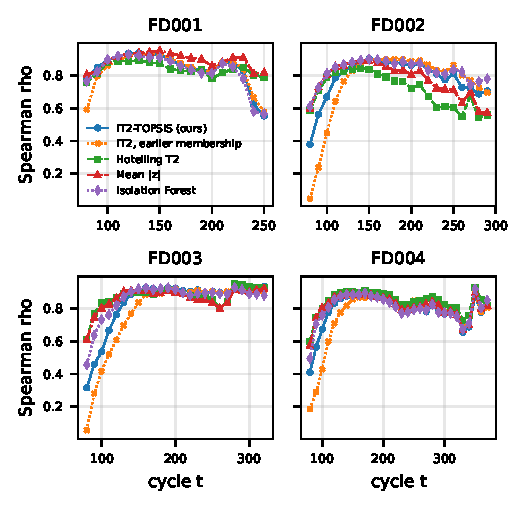
\includegraphics[width=\columnwidth]{figs/fig_rho_vs_t_v3.pdf}
\caption{Spearman $\rho$ per training batch on the four subsets. ``IT2, earlier membership'' is the earlier lower-membership formula inside the new pipeline.}
\label{fig:rho}
\end{figure}

\subsection{Held-out test engines}
\begin{table}[t]
\centering
\footnotesize
\caption{Test engines ranked at their last cycle: Spearman $\rho$ (R-precision in brackets for three methods). 95\% bootstrap intervals for IT2-TOPSIS: FD001 [.78,.91], FD002 [.85,.90], FD003 [.66,.85], FD004 [.74,.83].}
\label{tab:test}
\setlength{\tabcolsep}{3pt}
\begin{tabular}{lcccc}
\toprule
Method & FD001 & FD002 & FD003 & FD004 \\
\midrule
IT2-TOPSIS (ours) & .859 (.84) & .879 (.84) & .776 (.75) & .792 (.57) \\
Interval TOPSIS & .859 & .882 & .780 & .799 \\
Type-1 TOPSIS & .859 & .873 & .780 & .793 \\
Mean $|z|$ & .861 & .868 & .754 & .793 \\
Hotelling $T^2$ & .852 & .854 & .772 & .809 \\
Isolation Forest & .858 & .879 & .772 & .782 \\
PCA-SPE & .808 & .671 & .715 & .629 \\
Ridge index (sup.) & .860 (.88) & .907 (.89) & .895 (.85) & .886 (.85) \\
Age only & .601 (.48) & .702 (.46) & .551 (.50) & .452 (.30) \\
\bottomrule
\end{tabular}
\end{table}
On the test engines (Table~\ref{tab:test}) all unsupervised rankers except PCA-SPE lie within about 0.03 of each other on every subset, and all are far above the age-only ranker (0.45 to 0.70), so their skill does not come from how long an engine has been observed. The supervised ridge index matches them on FD001 but is clearly better on FD002 to FD004 ($\rho$ 0.89 to 0.91, R-precision 0.85 to 0.89 against 0.57 to 0.84 for IT2-TOPSIS), most of all on the two-fault subsets. Where run-to-failure labels exist, a supervised health index is the stronger ranker; the unsupervised operators are useful when such labels are not available. A short test trajectory overlaps the per-engine reference period and therefore looks healthy; this usually ranks it correctly, because short trajectories tend to have high RUL, and it affects all per-engine methods equally.

\subsection{Sensitivity}
\begin{figure}[t]
\centering
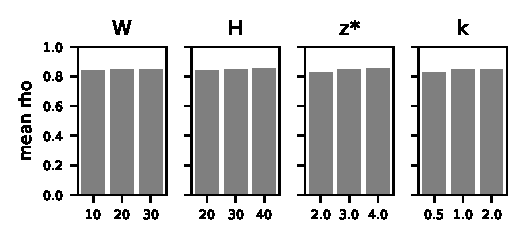
\includegraphics[width=\columnwidth]{figs/fig_sensitivity_v3.pdf}
\caption{FD001: mean training $\rho$ of IT2-TOPSIS when one parameter is varied and the others are at default.}
\label{fig:sens}
\end{figure}
On FD001, varying one parameter at a time (Fig.~\ref{fig:sens}) moves mean $\rho$ between 0.827 and 0.857: $W\in\{10,20,30\}$ gives 0.841, 0.846, 0.850; $H\in\{20,30,40\}$ gives 0.840, 0.846, 0.853; $z_\star\in\{2,3,4\}$ gives 0.827, 0.846, 0.857; $k\in\{0.5,1,2\}$ gives 0.830, 0.846, 0.849. A larger $z_\star$ helps because fewer upper memberships saturate at 1.

\subsection{What the FOU width detects}
\label{sec:fault}
No subset contains labelled sensor faults, so we inject them. Engines in the first half of each training set provide clean cells for a threshold at a 1\% false-alarm rate. For the other engines, in every batch one random sensor per engine receives one of four faults in the raw window: a noise burst ($N(0,(2\sigma^{\mathrm h})^2)$ on the last 10 readings), a bias step ($\pm3\sigma^{\mathrm h}$ on the last 10), a spike ($\pm8\sigma^{\mathrm h}$ on one reading) or a zero-mean variance increase ($N(0,(1.5\sigma^{\mathrm h})^2)$ over the whole window with its sample mean removed, so the window mean is unchanged). We compare the FOU width with the upper membership alone, a mean-plus-spread score $|z|+k\,s/\sigma^{\mathrm h}$, the rolling spread ratio $s/\sigma^{\mathrm h}$, the detrended spread ratio $r/\sigma^{\mathrm h}$ and a bootstrap interval width of the window mean. Table~\ref{tab:fault} reports the area under the ROC curve (AUC), the standardised partial AUC for false-alarm rates up to 5\%, and the detection rate at a threshold set for a realised 1\% false-alarm rate on the evaluated engines, averaged over the four subsets and four fault types.

\begin{table}[t]
\centering
\footnotesize
\caption{Injected sensor faults, averaged over four subsets and four fault types. TPR@1\%: detection rate at 1\% realised false alarms. Last two columns: TPR@1\% for bias steps and zero-mean variance faults.}
\label{tab:fault}
\setlength{\tabcolsep}{2.5pt}
\begin{tabular}{lccccc}
\toprule
Detector & AUC & pAUC & TPR@1\% & Bias & Var. \\
\midrule
FOU width, detrended (ours) & .78 & .67 & .27 & .07 & .31 \\
FOU width, raw $s$ & .81 & .70 & .34 & .38 & .31 \\
Upper membership & .70 & .51 & .00 & .00 & .00 \\
Mean plus spread & .72 & .50 & .01 & .01 & .01 \\
Rolling spread ratio & .97 & .75 & .18 & .16 & .15 \\
Detrended spread ratio & .94 & .79 & .39 & .07 & .42 \\
Bootstrap CI width & .96 & .74 & .17 & .15 & .15 \\
\bottomrule
\end{tabular}
\end{table}
Three conclusions follow. First, detectors driven by the window mean (upper membership, mean plus spread) detect almost nothing at a 1\% false-alarm rate, because degraded engines already produce large mean deviations; the FOU signal therefore does not come from mean shift. Second, the FOU width is not a better detector than the spread statistic it is built from: the detrended spread ratio has higher AUC (0.94 against 0.78), higher partial AUC and a higher detection rate at 1\% false alarms. The clipping and the zero floor of the membership map discard part of the spread information. Third, detrending trades bias steps for noise: it removes most of a step in the second half of the window, so the raw-spread FOU detects bias steps (0.38) where the detrended statistics do not. In practice a monitoring layer should flag channels with the detrended spread ratio, use the raw spread for steps, and use the FOU for what it does well: showing the operator, on the same $[0,1]$ urgency scale as the ranking, how wide the plausible urgency of each channel is.

\subsection{Packet loss and noise}
On FD001 we drop each record independently with probability $p$, add $N(0,(0.1\sigma^{\mathrm h})^2)$ to the remaining readings, and require at least $W/2$ readings per window (three seeds, all batches). For $p=0.1,0.2,0.3$ the Kendall $\tau$ between the IT2 rank and the clean rank is 0.967, 0.947 and 0.934, and $\rho$ against RUL stays at 0.846, 0.844 and 0.842; at most 1.8\% of engines lose their window. Mean directional $z$ and Hotelling $T^2$ are slightly more stable ($\tau$ 0.946 and 0.950 at $p=0.3$) and Isolation Forest slightly less (0.929).

\subsection{Tightness of the delay bounds}
\label{sec:delay}
For each training batch we rank with all windows delayed by $\tau$ cycles and compare the largest observed $|C_i(t)-C_i(t-\tau)|$ with two bounds: Proposition~\ref{p:lip} with $\delta$ measured from the membership endpoints, and Proposition~\ref{p:delay} with $D^m_j$ and $D^r_j$ measured as the largest change of the window mean and detrended spread. Both bounds hold in every batch of every subset. For $\tau\in\{1,2,5\}$ the first is 11 to 24 times the observed change (FD001: 0.44, 0.51 and 0.79 against 0.025, 0.036 and 0.069) and the second 26 to 43 times. The bounds assume that all $2m$ endpoints move adversarially at once; they are safe worst cases for choosing a watermark, not forecasts.

\subsection{Streaming replay and cost}
We replay the 20\,631 FD001 training rows record by record in cycle order with the sliding update of Section~\ref{sec:stream} and rank the live engines at the end of each cycle. In Python with NumPy on one core the replay processes about 36\,000 records per second; the per-cycle ranking takes 1.2\,ms at the median and 2.4\,ms at the 99th percentile (312 cycles); and the incremental detrended spread matches a batch recomputation to $1.2\times10^{-14}$. The vectorised ranking kernel takes 0.27\,ms, 6.2\,ms and 82\,ms for $10^3$, $10^4$ and $10^5$ assets with $m=14$. At these fleet sizes one process suffices.

\section{Discussion and limitations}
Across all four C-MAPSS subsets the evidence supports a narrow claim. A carefully built windowed IT2-TOPSIS operator is a sound, reproducible and competitive unsupervised ranker. It is within 0.05 of the best unsupervised method on every subset, but no unsupervised method wins consistently, and a supervised health index is clearly better where labels exist. Its distinctive output, the FOU interval, is an interpretable presentation of spread on the urgency scale, not a superior fault detector: a detrended spread ratio flags faults better. The two choices that mattered most, a per-asset healthy reference and a correct lower membership, are cheap and transfer to any method.

Limitations:
\begin{itemize}
\item All data are simulated; faults are injected synthetically and of four simple types. N-CMAPSS~\cite{arias2021} and field data with labelled sensor faults would be stronger tests.
\item Sensors are used as criteria with equal weights; a real cost, safety and throughput trade-off would need elicited weights and criteria beyond raw sensors.
\item The healthy reference is frozen after $H$ cycles, and operating conditions are handled by a fixed clustering of the training settings.
\item The delay bounds are loose by one to two orders of magnitude.
\item The streaming replay runs in one process; no Spark or Flink deployment was measured.
\end{itemize}

\section{Conclusion}
We corrected and evaluated a windowed IT2-TOPSIS operator for fleet condition monitoring on all four C-MAPSS subsets. A lower membership defined as the distance from zero to the standardised interval and a per-asset healthy reference give significant, consistent gains over the earlier operator. With them the operator ranks engines about as well as interval TOPSIS, type-1 TOPSIS, Hotelling $T^2$, Isolation Forest and the mean absolute $z$-score, never best and never far behind, and below a supervised health index on the harder subsets. Its FOU interval places channel spread on the urgency scale for the operator, but a plain detrended spread ratio is the better fault flag. The operator runs incrementally at $O(m)$ per record and its closeness coefficient obeys verified, if conservative, stability bounds.

\section*{Declarations}
\textbf{Data.} NASA C-MAPSS FD001 to FD004 (training, test and RUL files), public~\cite{saxena2008}. \textbf{Code.} \texttt{code/it2\_stream\_v3.py} (which imports the model from \texttt{it2\_stream\_v2.py}) produces every number, table and figure in this version (\texttt{results/metrics\_v3.json}, about 6 minutes on one core); seeds 0, 7, 11, 23, 41 and 2026. Scripts of earlier versions are kept for comparison. \textbf{Author contributions.} M.S.R.\ and N.Y.: formulation and proofs. A.M.\ and A.A.: software, experiments, figures. All authors reviewed the manuscript. \textbf{Conflict of interest.} None. \textbf{Funding.} None reported.

\begin{thebibliography}{50}
\bibitem{hwang1981}
C.-L. Hwang and K. Yoon, \emph{Multiple Attribute Decision Making: Methods and Applications}. Berlin, Germany: Springer, 1981.
\bibitem{chen2000}
C.-T. Chen, ``Extensions of the TOPSIS for group decision-making under fuzzy environment,'' \emph{Fuzzy Sets Syst.}, vol.\ 114, no.\ 1, pp.\ 1-9, 2000.
\bibitem{chen2010it2}
S.-M. Chen and L.-W. Lee, ``Fuzzy multiple attributes group decision-making based on the interval type-2 TOPSIS method,'' \emph{Expert Syst. Appl.}, vol.\ 37, no.\ 4, pp.\ 2790-2798, 2010.
\bibitem{celik2015}
E. \c{C}elik, M. Gul, N. Aydin, A.~T. Gumus, and A.~F. Guneri, ``A comprehensive review of multi criteria decision making approaches based on interval type-2 fuzzy sets,'' \emph{Knowl.-Based Syst.}, vol.\ 85, pp.\ 329-341, 2015.
\bibitem{macgregor1995}
J.~F. MacGregor and T. Kourti, ``Statistical process control of multivariate processes,'' \emph{Control Eng. Pract.}, vol.\ 3, no.\ 3, pp.\ 403-414, 1995.
\bibitem{liu2008iforest}
F.~T. Liu, K.~M. Ting, and Z.-H. Zhou, ``Isolation forest,'' in \emph{Proc. IEEE ICDM}, 2008, pp.\ 413-422.
\bibitem{saxena2008}
A. Saxena, K. Goebel, D. Simon, and N. Eklund, ``Damage propagation modeling for aircraft engine run-to-failure simulation,'' in \emph{Proc. Int. Conf. Prognostics Health Manage. (PHM)}, Denver, CO, USA, 2008.
\bibitem{zadeh1975}
L.~A. Zadeh, ``The concept of a linguistic variable and its application to approximate reasoning, I,'' \emph{Inf. Sci.}, vol.\ 8, no.\ 3, pp.\ 199-249, 1975.
\bibitem{liang2000}
Q. Liang and J.~M. Mendel, ``Interval type-2 fuzzy logic systems: Theory and design,'' \emph{IEEE Trans. Fuzzy Syst.}, vol.\ 8, no.\ 5, pp.\ 535-550, Oct. 2000.
\bibitem{mendel2002}
J.~M. Mendel and R.~I. John, ``Type-2 fuzzy sets made simple,'' \emph{IEEE Trans. Fuzzy Syst.}, vol.\ 10, no.\ 2, pp.\ 117-127, Apr. 2002.
\bibitem{mendel2006}
J.~M. Mendel, R.~I. John, and F. Liu, ``Interval type-2 fuzzy logic systems made simple,'' \emph{IEEE Trans. Fuzzy Syst.}, vol.\ 14, no.\ 6, pp.\ 808-821, Dec. 2006.
\bibitem{mendel2017}
J.~M. Mendel, \emph{Uncertain Rule-Based Fuzzy Systems: Introduction and New Directions}, 2nd ed. Cham, Switzerland: Springer, 2017.
\bibitem{karnik2001}
N.~N. Karnik and J.~M. Mendel, ``Centroid of a type-2 fuzzy set,'' \emph{Inf. Sci.}, vol.\ 132, no.\ 1-4, pp.\ 195-220, 2001.
\bibitem{wu2002}
H. Wu and J.~M. Mendel, ``Uncertainty bounds and their use in the design of interval type-2 fuzzy logic systems,'' \emph{IEEE Trans. Fuzzy Syst.}, vol.\ 10, no.\ 5, pp.\ 622-639, Oct. 2002.
\bibitem{nie2008}
M. Nie and W.~W. Tan, ``Towards an efficient type-reduction method for interval type-2 fuzzy logic systems,'' in \emph{Proc. IEEE Int. Conf. Fuzzy Syst. (FUZZ-IEEE)}, 2008, pp.\ 1425-1432.
\bibitem{bustince2016}
H. Bustince \emph{et al.}, ``A historical account of types of fuzzy sets and their relationships,'' \emph{IEEE Trans. Fuzzy Syst.}, vol.\ 24, no.\ 1, pp.\ 179-194, Feb. 2016.
\bibitem{kahraman2014}
C. Kahraman, B. \"Oztay\c{s}i, \.{I}. U\c{c}al Sari, and E. Turano\u{g}lu, ``Fuzzy analytic hierarchy process with interval type-2 fuzzy sets,'' \emph{Knowl.-Based Syst.}, vol.\ 59, pp.\ 48-57, 2014.
\bibitem{qin2015}
J. Qin and X. Liu, ``Multi-attribute group decision making using combined ranking value under interval type-2 fuzzy environment,'' \emph{Inf. Sci.}, vol.\ 297, pp.\ 293-315, 2015.
\bibitem{jahanshahloo2006}
G.~R. Jahanshahloo, F. Hosseinzadeh Lotfi, and M. Izadikhah, ``An algorithmic method to extend TOPSIS for decision-making problems with interval data,'' \emph{Appl. Math. Comput.}, vol.\ 175, no.\ 2, pp.\ 1375-1384, 2006.
\bibitem{dymova2013}
L. Dymova, P. Sevastjanov, and A. Tikhonenko, ``A direct interval extension of TOPSIS method,'' \emph{Expert Syst. Appl.}, vol.\ 40, no.\ 12, pp.\ 4841-4847, 2013.
\bibitem{opricovic2004}
S. Opricovic and G.-H. Tzeng, ``Compromise solution by MCDM methods: A comparative analysis of VIKOR and TOPSIS,'' \emph{Eur. J. Oper. Res.}, vol.\ 156, no.\ 2, pp.\ 445-455, 2004.
\bibitem{behzadian2012}
M. Behzadian, S. Khanmohammadi Otaghsara, M. Yazdani, and J. Ignatius, ``A state-of-the-art survey of TOPSIS applications,'' \emph{Expert Syst. Appl.}, vol.\ 39, no.\ 17, pp.\ 13051-13069, 2012.
\bibitem{liao2015}
H. Liao, Z. Xu, and X.-J. Zeng, ``Hesitant fuzzy linguistic VIKOR method and its application in qualitative multiple criteria decision making,'' \emph{IEEE Trans. Fuzzy Syst.}, vol.\ 23, no.\ 5, pp.\ 1343-1355, 2015.
\bibitem{saaty1980}
T.~L. Saaty, \emph{The Analytic Hierarchy Process}. New York, NY, USA: McGraw-Hill, 1980.
\bibitem{chang1996}
D.-Y. Chang, ``Applications of the extent analysis method on fuzzy AHP,'' \emph{Eur. J. Oper. Res.}, vol.\ 95, no.\ 3, pp.\ 649-655, 1996.
\bibitem{babcock2002}
B. Babcock, S. Babu, M. Datar, R. Motwani, and J. Widom, ``Models and issues in data stream systems,'' in \emph{Proc. PODS}, 2002, pp.\ 1-16.
\bibitem{stonebraker2005}
M. Stonebraker, U. \c{C}etintemel, and S. Zdonik, ``The 8 requirements of real-time stream processing,'' \emph{SIGMOD Rec.}, vol.\ 34, no.\ 4, pp.\ 42-47, 2005.
\bibitem{zaharia2013}
M. Zaharia \emph{et al.}, ``Discretized streams: Fault-tolerant streaming computation at scale,'' in \emph{Proc. SOSP}, 2013, pp.\ 423-438.
\bibitem{carbone2015}
P. Carbone \emph{et al.}, ``Apache Flink: Stream and batch processing in a single engine,'' \emph{IEEE Data Eng. Bull.}, vol.\ 38, no.\ 4, pp.\ 28-38, 2015.
\bibitem{akidau2015}
T. Akidau \emph{et al.}, ``The dataflow model: A practical approach to balancing correctness, latency, and cost in massive-scale, unbounded, out-of-order data processing,'' \emph{Proc. VLDB Endow.}, vol.\ 8, no.\ 12, pp.\ 1792-1803, 2015.
\bibitem{gama2014}
J. Gama, I. Zliobaite, A. Bifet, M. Pechenizkiy, and A. Bouchachia, ``A survey on concept drift adaptation,'' \emph{ACM Comput. Surv.}, vol.\ 46, no.\ 4, 2014, Art.\ no.\ 44.
\bibitem{bifet2010}
A. Bifet, G. Holmes, R. Kirkby, and B. Pfahringer, ``MOA: Massive online analysis,'' \emph{J. Mach. Learn. Res.}, vol.\ 11, pp.\ 1601-1604, 2010.
\bibitem{kasabov2002}
N. Kasabov and Q. Song, ``DENFIS: Dynamic evolving neural-fuzzy inference system and its application for time-series prediction,'' \emph{IEEE Trans. Fuzzy Syst.}, vol.\ 10, no.\ 2, pp.\ 144-154, Apr. 2002.
\bibitem{angelov2004}
P. Angelov and D. Filev, ``An approach to online identification of Takagi-Sugeno fuzzy models,'' \emph{IEEE Trans. Syst., Man, Cybern. B}, vol.\ 34, no.\ 1, pp.\ 484-498, Feb. 2004.
\bibitem{lughofer2011}
E. Lughofer, \emph{Evolving Fuzzy Systems: Methodologies, Advanced Concepts and Applications}. Berlin, Germany: Springer, 2011.
\bibitem{welford1962}
B.~P. Welford, ``Note on a method for calculating corrected sums of squares and products,'' \emph{Technometrics}, vol.\ 4, no.\ 3, pp.\ 419-420, 1962.
\bibitem{arias2021}
M. Arias Chao, C. Kulkarni, K. Goebel, and O. Fink, ``Aircraft engine run-to-failure dataset under real flight conditions for prognostics and diagnostics,'' \emph{Data}, vol.\ 6, no.\ 1, Art.\ no.\ 5, 2021.
\bibitem{wang2008}
T. Wang, J. Yu, D. Siegel, and J. Lee, ``A similarity-based prognostics approach for remaining useful life estimation of engineered systems,'' in \emph{Proc. Int. Conf. Prognostics Health Manage.}, 2008.
\bibitem{babu2016}
G.~S. Babu, P. Zhao, and X.-L. Li, ``Deep convolutional neural network based regression approach for estimation of remaining useful life,'' in \emph{Proc. DASFAA}, 2016, pp.\ 214-228.
\bibitem{li2018}
X. Li, Q. Ding, and J.-Q. Sun, ``Remaining useful life estimation in prognostics using deep convolution neural networks,'' \emph{Reliab. Eng. Syst. Saf.}, vol.\ 172, pp.\ 1-11, 2018.
\bibitem{zheng2017}
S. Zheng, K. Ristovski, A. Farahat, and C. Gupta, ``Long short-term memory network for remaining useful life estimation,'' in \emph{Proc. IEEE ICPHM}, 2017, pp.\ 88-95.
\bibitem{lei2018}
Y. Lei, N. Li, L. Guo, N. Li, T. Yan, and J. Lin, ``Machinery health prognostics: A systematic review from data acquisition to RUL prediction,'' \emph{Mech. Syst. Signal Process.}, vol.\ 104, pp.\ 799-834, 2018.
\bibitem{sikorska2011}
J.~Z. Sikorska, M. Hodkiewicz, and L. Ma, ``Prognostic modelling options for remaining useful life estimation by industry,'' \emph{Mech. Syst. Signal Process.}, vol.\ 25, no.\ 5, pp.\ 1803-1836, 2011.
\bibitem{ramasso2014}
E. Ramasso and A. Saxena, ``Performance benchmarking and analysis of prognostic methods for CMAPSS datasets,'' \emph{Int. J. Prognostics Health Manage.}, vol.\ 5, no.\ 2, 2014.
\bibitem{efron1993}
B. Efron and R.~J. Tibshirani, \emph{An Introduction to the Bootstrap}. New York, NY, USA: Chapman \& Hall, 1993.
\bibitem{angelopoulos2023}
A.~N. Angelopoulos and S. Bates, ``Conformal prediction: A gentle introduction,'' \emph{Found. Trends Mach. Learn.}, vol.\ 16, no.\ 4, pp.\ 494-591, 2023.
\end{thebibliography}
\end{document}
